\chapter{Introduction}
\label{chap:introduction}

In our modern society, the authentication procedure is an important task to protect data and resources (physical or digital). Consisting of the confirmation of a claimed identity, the authentication step is the first and most critical task of security procedure, restricting access to unauthorized users. 

Biometrics is the science of recognizing the identity of a person based on their physical attributes and / or behavior, such as face, fingerprints, hand veins, voice or iris \cite{li2011handbook}. The use of biometrics in an authentication procedure has some advantages. Naturally, is not possible to forget or transfer a biometric trait and it hardly disappears (perhaps only in case of a seriously accidents). However, biometrics has some drawbacks. Compared with regular authentication systems, such as passwords or tokens, which are precise, biometric authentication systems have probabilistic behavior. It turns out that biometrics hardly has perfect match; therefore, authentication systems have to deal with error rates. These errors rates can vary depending on a number of factors. As an example, our voice can vary drastically  when we get sick or when we are under stress and this impacts a speaker authentication system. Aging, illumination, pose and face expressions are classical issues in face authentication systems.


The use of biometrics in our daily lives has grown in the last decade and we can quote several examples of this. The confirmation of an identity in the brazilian electoral process is based on fingerprints. In Brazil, a bank replaced the use of passwords to palm vein authentication in ATMs. The demand for security pushes the market towards biometrics. A recent marked research estimates that the overall market for voice and face biometrics is expected to reach nearly US\$3 billions by the end of 2018\footnote{\url{http://www.biometricupdate.com/201307/voice-biometrics-and-how-far-weve-come/?goback=\%2Egde\_40210\_member\_258411747}}.


A biometric authentication system can be represented with the simple flow chart in Figure \ref{fig:diagram_attacks}.

\begin{figure}[!htb]
\begin{center}
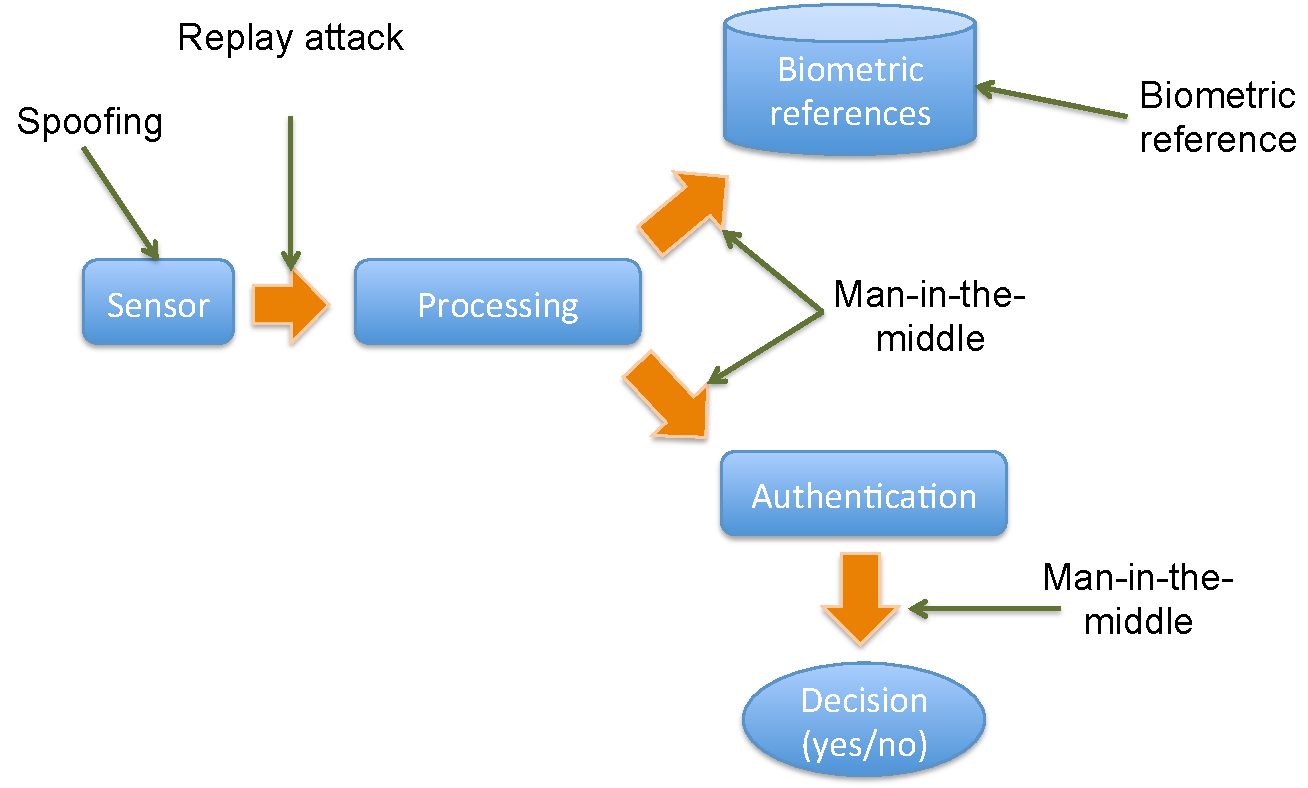
\includegraphics [width=14cm] {images/diagram_attacks.pdf}
\caption[Simple architecture of a regular biometric authentication system]{Simple architecture of a regular biometric authentication system (adapted from \cite{xiao2005security})} \label{fig:diagram_attacks}
\end{center}
\end{figure}

Firstly, the biometric trait is captured using some kind of sensor. Secondly, the captured biometric trait is processed in order to extract biometric features. When it is in an enrollment procedure, these features will generate a biometric reference, and will be stored in a database. In an authentication procedure, these features will be compared with the stored biometric reference. It is possible to observe, in the same Figure, that attacks can be done at any point of the architecture \cite{xiao2005security}. 
%The next subsections discuss each one of the possible points of attack and how to mitigate it.

%\subsection{Replay attack}
%\label{sec:rep}

The \textbf{replay attack} is performed by injecting a biometric data, of the target identity, previously captured in order to gain a non authorized access. The biometric data can be obtained sniffing the biometric authentication software. To mitigate this kind of attack, the biometric system should ensure that the provided data was not injected artificially \cite{xiao2005security}. A common way to protect against this kind of attack is to associate a timestamp to the data. As it is improbable to have exactly the same biometric data in different times, this method can be quite effective.

%\subsection{Biometric reference attack}

The \textbf{biometric reference attack} is performed where the biometrics are stored. This kind of attack, include actions such as the inclusion, removal, modification and theft biometric references. Among this actions, the possibility to steal a biometric reference is the most dangerous threat, since it is possible to work in a reverse engineering process to regenerate the biometric trait. 

Using a hill climbing technique to optimize to the position and the orientation of the minutia \cite{MartinezDiaz2006} and \cite{hill2001risk} show that is possible to generate synthetic fingerprints compatible with fingerprints stored in a database. Fake fingers (with a real fingerprint) made of gummy or silicone can be generated with this minutia. It is possible also to inject these minutia in the \textbf{Processing} module (see Figure \ref{fig:diagram_attacks}) in order to deceive the authentication system. 

To mitigate the risk of this kind of attack, best practices in security recommend to encrypt the biometric references and to increase the security policies to access these biometric references. 

%\subsection{Man-in-the-middle}

In the \textbf{man in the middle attack}, the biometric data is intercepted in any point of the architecture in Figure \ref{fig:diagram_attacks}.  As shown in the Figure \ref{fig:diagram_attacks}, the attacker can:
\begin{itemize}
        \item Manipulate the matching score;
        \item Manipulate the biometric authentication response;
        \item Steal biometric data;
        \item Inject biometric data.
\end{itemize}

The same security recommendations aforementioned to deal with this security breaks can be used here; i.e. encrypt the data before transmission, increase the security grants and so on. 

%\subsection{Ataque de Spoofing}

The \textbf{spoofing attack}, in biometric systems, is a direct attack to the biometric sensor; i.e. a forged biometric trait is presented to the biometric sensor in order to deceive the system. The goal is to pretend to be someone else in order to get forbidden privileges. Most biometric systems can be spoofed. Next subsections presents a brief discussion about spoofing in different biometric traits:

\subsubsection{Fingerprint}

In fingerprints verification systems, the attacker can forge a fingerprint with different materials (gummy, silicone, etc). \cite{matsumoto2002impact} and \cite{leyden2002gummi} discuss how to generate fake fingerprints using materials easily found in supermarkets. Figure \ref{fig:finger_attack} shows how easy is to create a molds from a live fingers and to reproduce its fingerprints with gummy. This fake fingers can be used  to spoof a fingerprint biometric systems.

\begin{figure}[!htb]
\begin{center}
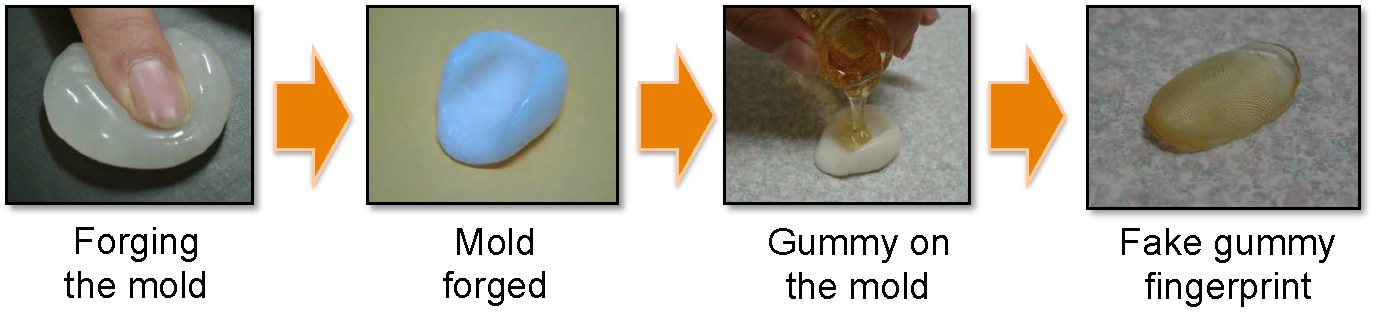
\includegraphics [width=16cm] {images/finger_print_attack.pdf}
\caption[Creating a fake fingerprint]{Creating a fake fingerprint (Adapted from \cite{matsumoto2002impact})} \label{fig:finger_attack}
\end{center}
\end{figure}

Recently in Brazil (2013), it was reported that doctors in S\~ao Paulo were arrested after being caught in the act of using fake fingers made of silicone and imprinted with real fingerprints to defraud a hospital's biometric punch-in clock\footnote{\url{http://www.foxnews.com/us/2013/03/13/brazilian-doctors-use-fake-silicone-fingers-to-defraud-hospital-punch-in-clock/}}.

%A more sophisticated attack is discussed in \cite{MartinezDiaz2006} and \cite{hill2001risk}. These papers use a hill climbing technique to optimize  the position and the orientation of the minutia. With this optimization was possible to generate fingerprints compatible for match.

%Using a hill climbing technique to optimize to the position and the orientation of the minutia  shown that is possible to generate fingerprints compatible with fingerpri
%A more sophisticated attack were discussed in \cite{uludag2004attacks}. This paper uses a hill climbing procedure to optimize the position and the orientation of the minutia in a minutia based fingerprint verification system. The optimized result of the minutia can be used to generate a fake finger.

%FALAR DOS SENSORES.

%http://www.tabularasa-euproject.org/news/selected-news-related-to-spoofing-attacks

\subsubsection{Speaker}

For speech biometrics, the attacker can forge a human voice by mimicry or recording the voice of the target identity and replaying it back to the microphone. 

\cite{chetty2004liveness} and \cite{eveno2005speaker} address the problem using audio-visual features. The first one proposes a bi-modal authentication system using the face information in order to increase security. The second one correlates the lip movements with the content of the speech as a security barrier.

\cite{QimingZhu} analyse the speech signal itself applying the 1-dimensional $LBP$ (Local Binary Pattern) followed by a SVM (Support Vector Machines) in order to detect spoofs.

\subsubsection{Iris}

Iris biometrics has traditionally been regarded as one of the most reliable and accurate biometric traits, but as the other biometric traits it can also be spoofed. A simple way to spoof an iris recognition system is using a high quality printed image. More sophisticated attacks using contact lenses can also be carried out.

Countermeasures to deal with this kind of attacks can be deployed in hardware (with a specific equipment) or in the software \cite{Galbally_ICB-2012}. Especially in the software level, \cite{Galbally_ICB-2012} address the problem using various types of features, including a set of  high pass filters, motion features and occlusion filters in the iris images followed by a binary classifier as countermeasure. 

An approach based on textures was carried out by \cite{ZhuoshiWei}. This countermeasure uses the co-occurrence matrix descriptor followed by a binary classifier.

%Measuring the pupil reflex using a set of high filters, \cite{kanematsu2007highly}
% \cite{johnson2010multimodal}, \cite{kanematsu2007highly} and \cite{pacut2006aliveness} are works addressing spoofing attacks in iris biometric system. 

\subsubsection{Face}

Recently, the media has reported some situations of attacks in deployed face recognition systems. Using simple photographs, a research group from University of Hanoi showed how easy is to spoof the face authentication systems deployed in Lenovo, Asus and Toshiba Laptops \cite{BlackHat2009}. Since the release \textit{Ice Cream Sandwich}, the Android OS come with a built-in face authentication system to unlock the mobile phone. Since then, it has been extensively demonstrated around the web how easy it is to spoof this face recognition system\footnote{\url{http://www.itproportal.com/2011/11/14/ice-cream-sandwich-facial-recognition-cracked/}}. As a consequence, an eye blinking detection has been introduced in the most recent version of the Android OS. Spoofing in face authentication will be discussed in details in the Chapter \ref{chap:Spoofing}. \\ \\ 

Several technologies related to information security can be deployed in a biometric authentication systems in order to mitigate the mentioned attacks. We can highlight:
\begin{itemize}
        \item Encrypt the biometric data;
        \item Improve the security policies;
        \item Convey the biometric data using a secure channel;
        \item Deploy all modules of the architecture in a physical arrangement that cannot be penetrated;
        \item Using more than one authentication factor.
\end{itemize}
However, in a spoofing attack, the target is the biometric sensor, and in the architecture presented in Figure \ref{fig:diagram_attacks}, is not possible to apply any of the security tools to prevent this kind of attack, becoming the most fragile point. To mitigate this kind of vulnerability, effective countermeasures against spoofing have to be deployed.


\section{Scope and Contributions}
\label{sec:scope}

Focusing in antispoofing countermeasures for face authentication, the goal of this masters dissertation is two fold. The first one, we introduce a novel method to detect face spoofing using the spatiotemporal (dynamic texture) extensions of the Local Binary Pattern. The key idea of the approach is to learn and detect the structure and the dynamics of the facial micro-textures that characterises real faces but not fake ones. The second one, is to provide a comparative study of state of the art countermeasures for face antispoofing. The key contribution of this comparative study is to cover tests in all video face antispoofing databases freely available focusing in the biases that these databases can introduce in the countermeasures.

\section{Organization of the Masters Dissertation}
\label{sec:scope}

Besides this introduction, that presented the motivation of this work, the dissertation has four more chapters. 

The Chapter \ref{chap:Spoofing} defines spoofing attacks in face authentication, presenting the main countermeasures and databases available for this research.

The Chapter \ref{chap:Proposed_Countermeasures} defines and presents the results of the proposed countermeasure based on dynamic texture, the first contribution of this dissertation and their results.

The Chapter \ref{chap:Comparative_Study} defines and presents the results of the comparative study of face antispoofing countermeasures, the second contribution of this dissertation.

Finally, Chapter \ref{chap:Conclusions} presents the conclusions and future work.
